\chapter{ИССЛЕДОВАТЕЛЬСКИЙ РАЗДЕЛ}\label{ch:ch1}
Сертификация программного обеспечения проводится, 
когда необходимо подтвердить соответствие разрабатываемой 
продукции требованиям защиты информации.
Частым объектом сертификации является ПО, разработанное:
\begin{itemize}
    \item для обеспечения информационной безопасности;
    \item для осуществления коммуникации между людьми или программно-аппаратными~комплексами;
    \item для техники военного назначения;
    \item крупными разработчиками программного обеспечения.
\end{itemize}

Подтверждение безопасности программного обеспечения -- важный этап 
в продвижении программного продукта.

Сертификация не является универсальным способом 
решения всех существующих проблем в 
области информационной безопасности, однако 
сегодня это единственный реально функционирующий 
механизм, который обеспечивает независимый 
контроль качества средств защиты информации.
При грамотном применении механизм сертификации 
позволяет достаточно успешно решать задачу 
достижения гарантированного уровня защищенности автоматизированных систем.

{\actuality} Отсутствие недекларированных возможностей в скомпилированном
объектном файле является ключевым аспектом сертификации ПО.
Сертификация программного обеспечения необходима для 
подтверждения требований заказчика к защите 
информации, к выполнению функциональных 
и технических задач и к обеспечению работы ПО в целом.

\begin{figure}[!htbp]
    \centerfloat{
        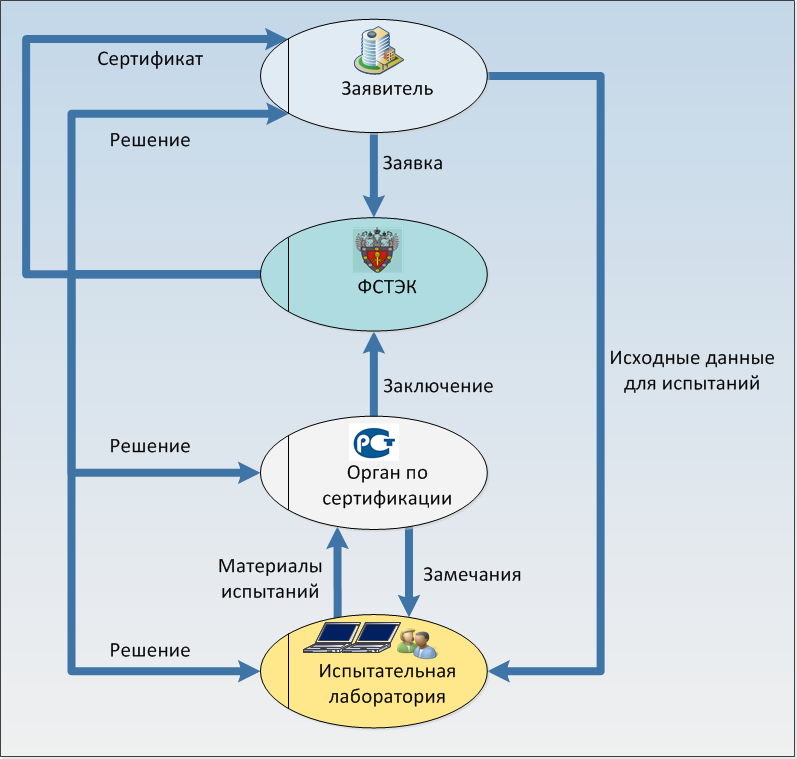
\includegraphics[width=\linewidth]{images/certification.png}
    }
    \caption{Процесс сертификации программного обеспечения во ФСТЭК\label{fig:fstak-cert}}
\end{figure}

Но существуют опасения, возникающие не на пустом месте,
что на любом из этапов сборки программы из
исходных кодов в ней может появиться программная 
закладка \autocite{compile-a-virus, ken-thompson-hack}.

Чтобы исключить подобные ситуации, применяется техника статического 
анализа исходных кодов, динамического анализа -- анализа пройденных 
программой трасс c последующим сравнением результатов статического и динамического анализов.

На данный момент не существует открытых программных решений,
позволяющих проводить сертификацию программного обеспечения в описанном ранее формате.
Самое близкое по назначению ПО -- это статические анализаторы \autocite{c-static-analysis},
и так использующиеся как составная часть в процессе сертификации.
Помимо них существует свободное программное обеспечение от корпорации Microsoft --
Microsoft Application Inspector \autocite{microsoft-application-inspector}, но оно
взаимодействует только с исходными кодами программы, распознавая паттерны и назначение
функций.
Помимо свободных программ существует утилита анализа ядра Linux от ООО Фирма <<Анкад>>. 
В ней проводится статический, динамический и сравнительный анализ, но программа не умеет
работать с чем либо, кроме ядра Linux и сертифицировать что-либо еще с помощью нее не получится.
На рисунке \ref{fig:fstak-cert} ООО Фирма <<Анкад>> выступает испытательной лабораторией.

Получается, что на рынке невозможно найти комбинированные решения, 
с помощью которого было бы возможно провести процесс сертификации любого ПО. 
Для каждого конкретного проекта приходится использовать различные статические анализаторы, 
динамические анализаторы, что приводит к дублированию кода и выполняемых действий, которые нужны для сертификации ПО.
Это ведет к разрастанию кодовой базы компании и нарастающим трудностям в последующей поддержке
каждого отдельного решения, что в свою очередь ведет к увеличению затрат компании.

Чтобы унифицировать разрабатываемое ПО для сертификации, было решено разбить {\ProgModule}
на модули, разделенные по ответственности и не знающие друг о друге. Это обеспечивает
удобство в редактировании, замене и изменении модулей, а при сохранении формата выдаваемой информации
 -- инкапсуляцию изменений только на конкретном модуле.

Так как модули не знают друг о друге, то и работают они в условиях ограниченной информации.
Модуль статического анализа обрабатывает только исходные коды, выдавая список статических
вызовов. Модуль динамического анализа работает с программой без отладочных символов,
собирая информацию на уровне машинных инструкций.

Данный подход помогает приблизить процесс сертификации к <<боевым>> условиям.

\section{Процесс сертификации ПО на отсутствие НДВ}\label{sec:ch1/sec1}
Сертификационная процедура состоит из следующих этапов:
\begin{enumerate}[label={\arabic*)}]
    \item готовность документации ПО, доступность исходных текстов;
    \item опредление объема исходных текстов, подлежащих анализу;
    \item обращение заявителя в испытательную лабораторию с собранной информацией;
    \item анализ документации;
    \item разработка <<Программы и методик проведения сертификационных испытаний>>;
    \item проведение испытаний;
    \item экспертиза результатов.
\end{enumerate}

Сертификация должна выявить присутствие в исполняемом файле недекларированных возможностей,
которые могут являться как злым умыслом разработчиков компилятора,
линкера и других вспомогательных программ, так и методами оптимизации ПО,
которые применяются для более рационального 
потребления ресурсов программой.

Впервые теоретическая возможность создания таких программ была описана
создателем языка Си, инженером Bell Labs -- Кеном Томпсоном в 1984 году,
в журнале ACM под названием <<Reflections on Trusting Trust>>
(<<Размышления о доверии>>) \autocite{ken-thompson-hack}.
В ней был описан компилятор, содержащий в себе следующий функционал:
\begin{itemize}
    \item компилятор знает, когда компилирует сторонние программы,
        а когда себя или другой компилятор;
    \item при компиляции любой программы, 
        в исполняемый файл внедряется некий вредоносный код;
    \item если компилятор компилирует себя или другой компилятор,
        то он добавляет функционал внедрения вредоносного кода в 
        другие компиляции программ и компилятора;
\end{itemize}

Такой компилятор разбивает уверенность в принципе, который можно описать
как <<я не доверяю скомпилированному бинарному файлу, я все собираю сам>>,
так как нельзя быть полностью уверенным, что 
в программе не появилось НДВ на стадии компиляции.

Эта статья так и оставалась бы чистым размышлением, если бы в 2009 году специалисты
из лаборатории по информационной безопасности -- SophosLabs не обнаружили компилятор
Delphi \autocite{compile-a-virus}, умеющий добавлять в исполняемые файлы вредоносную составляющую.
За день специалисты получили в свое распоряжение более 3000 уникальных исполняемых
файлов, зараженных W32/Induc-A. Это является серьезной угрозой безопасности, так как
распространителем вредоносных файлов может быть легитимный источник, например
известная компания по производству программного обеспечения.

Выявить данные расхождения между необработанными исходными кодами и 
поведением программы во время исполнения позволяет разработанный мной
программный модуль.

Дадим определение термину <<Недекларированные возможности>>.

\textbf{Недекларированные возможности} \autocite{undeclared-capabilities-antimalware} 
— намеренно измененная часть ПО, с помощью которой можно получить незаметный 
несанкционированный доступ к безопасной компьютерной среде.

\begin{figure}[!htbp]
    \centerfloat{
        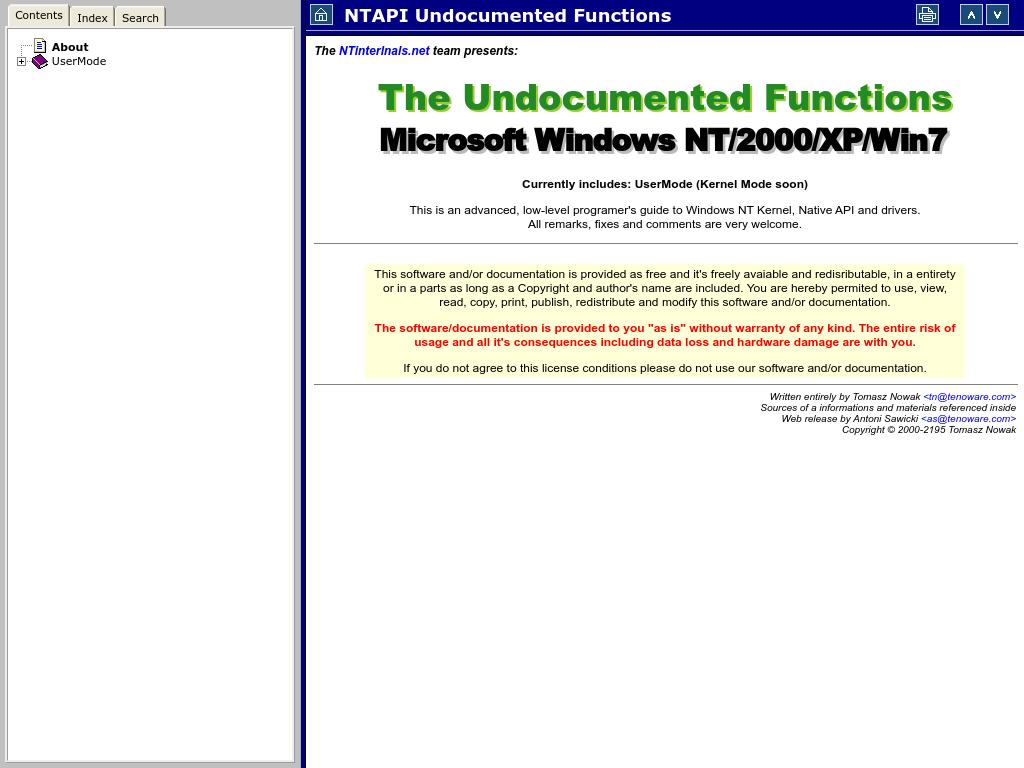
\includegraphics[width=\linewidth]{images/NTinternals.png}
    }
    \caption{Главная страница сайта NTinterlnals.net,
             на котором силами сообщества
             документировалось API Windows NT \label{fig:nt-internals}}
\end{figure}

\section{Классификация НДВ}\label{sec:ch1/sec2}
Классифицировать НДВ можно несколькими способами, в
зависимости от их целей для компрометации и способу использования.
    \subsection{По применению}\label{sec:ch1/sec2/sub1}
    Использование НДВ может реализовываться в:
    \begin{itemize}
        \item перехвате данных;
        \item подмене данных;
        \item выводе компьютерной системы из строя;
        \item полном доступе к удаленной компьютерной системе.
    \end{itemize}
    Причем при наличии полного доступа к компьютерной системе, вредоносные программы
    программы могут быть использованы злоумышленниками для
    всех вышеперечисленных целей.

\subsection{По целям}\label{sec:ch1/sec2/sub2}
Использование НДВ может быть направлено на различные типы целей, перечислим их
\begin{enumerate}[label={\arabic*)}]
    \item \textbf{Персональные компьютеры и рабочие станции}
          
          Целью могут быть как персональные компьютеры широкого числа пользователей,
          так и отдельные рабочие станции, которые могут являться точкой входа в
          защищенную компьютерную систему, так и использоваться для перехвата важной
          информации.
    \item \textbf{Серверы}
          
          Серверы обслуживают большое количество клиентов, а значит проникновение на
          сервер может существенно повлиять на работу всех компьютеров, работающих с
          данным сервером.
    \item \textbf{Встраиваемые системы}

          Благодаря постоянному удешелению микроконтроллеров и периферийных устройств,
          все больше и больше повседневных вещей обзаводятся <<умной>> функциональностью.
          Погоня производителей за прибылями отражается на безопасности прошивок умных устройств.
    \item \textbf{Промышленные компьютеры}

        Программные закладки в такие системы чреваты шпионажем или диверсией, как, например
        вирус Stuxnet\autocite{stuxnet}. Не смотря на то, что данная программа является вирусом, а
        не программой с НДВ, случившееся ярко показывает реальное применение подобных техник 
        для деструктивных действий.
\end{enumerate}

\section{Степень опасности НДВ}\label{sec:ch1/sec3}
Для определения опасности НДВ будем пользоваться следующими нормативными документами \autocite{fstec-21-blog}:
\begin{itemize}
    \item приказ ФСТЭК России от 18 февраля 2013 г. № 21;
    \item федеральный закон <<О персональных данных>> от 27.07.2006 N 152-ФЗ.
\end{itemize}

Тип угроз безопасности персональных данных определяется 
в зависимости от комбинаций критичности угроз в ИСПДн (\autoref{table:threats}):
\begin{itemize}
    \item наличием НДВ в системном программном обеспечении (ПО), используемом в ИСПДн;
    \item наличием НДВ в прикладном ПО, используемом в ИСПДн.
\end{itemize}

Согласно п.6 Требований к защите персональных данных при их обработке в ИСПДн,
утвержденных постановлением Правительства РФ от 01.11.2012 №1119 \autocite{privacy-protection},
установлены 3 типа актуальных угроз безопасности персональных данных.
Самый низкий тип угроз – третий, самый высокий – первый.
Они перечислены в таблице \ref{table:threats}. 

\begin{table}[!htbp]
    \centering
    \caption{\label{table:threats}Типы актуальных угроз}

    \begin{center}
        \begin{tabular}{ | c | c | c | c | }
            \hline
            Угрозы & \multicolumn{3}{ c |}{Тип актуальных угроз} \\
            \cline{2-4}
                   & 1 Тип & 2 Тип & 3 Тип\\
            \hline
            \makecell{Наличие НДВ в системном ПО,\\ используемом в ИСПДн} & \redcell{критично} & \greencell{некритично} & \greencell{некритично} \\
            \hline
            \makecell{Наличие НДВ в прикладном ПО \\ используемом в ИСПДн} & \makecell{критично \\ или \\ некритично} & \redcell{критично} & \greencell{некритично} \\
            \hline
        \end{tabular}
    \end{center}
\end{table}

Порядок определения актуальных угроз безопасности 
персональных данных в ИСПДн осуществляется 
в соответствии с Методикой определения 
актуальных угроз безопасности персональных данных 
при их обработке в информационных 
системах персональных данных, утвержденных 
ФСТЭК России, 2008 год.

Актуальной считается угроза, которая может быть 
реализована в ИСПДн и представляет опасность для 
персональных данных.  Подход к составлению перечня 
актуальных угроз состоит в следующем. 
Для оценки возможности реализации угрозы применяются два показателя: 

\begin{itemize}
    \item $Y_1$ - уровень исходной защищенности ИСПДн;
    \item $Y_2$ - частота (вероятность) реализации рассматриваемой угрозы;
\end{itemize}

Коэффициент реализуемости угрозы $Y$ определяется соотношением: 

\[Y = \frac{Y_1 + Y_2}{20}\]

По значению коэффициента реализуемости угрозы Y 
интерпретация реализуемости угрозы следующим образом: 
\begin{itemize}
    \item если $0 \leq Y \leq 0.3$, то возможность реализации угрозы признается низкой;
    \item если $0.3 < Y \leq  0.6$, то возможность реализации угрозы признается средней;
    \item если $0.6 < Y \leq  0.8$, то возможность реализации угрозы признается высокой;
    \item если $Y > 0,8$, то возможность реализации угрозы признается очень высокой.
\end{itemize}

Далее оценивается опасность каждой угрозы.
Этот показатель имеет три значения: 
\begin{itemize}
    \item низкая опасность – если реализация угрозы может привести к незначительным негативным последствиям для субъектов персональных данных;
    \item средняя опасность – если реализация угрозы может привести к негативным последствиям для субъектов персональных данных;
    \item высокая опасность – если реализация угрозы может привести к значительным негативным последствиям для субъектов персональных данных.
\end{itemize}

Затем осуществляется выбор из общего
перечня угроз безопасности тех, 
которые относятся к актуальным для данной ИСПДн,
в соответствии с правилами, приведенными в \autoref{table:actual-threats}
\begin{table}[!htbp]
    \centering
    %\captionsetup{justification=centering}
    \caption{\label{table:actual-threats}Правила отнесения угрозы безопасности персональных данных к критичной}

    \begin{center}
        \begin{tabular}{ | c | c | c | c | }
            \hline
            \makecell{Возможность \\ реализации угрозы} & \multicolumn{3}{ c |}{Показатель опасности угрозы} \\
            \cline{2-4}
                   & Низкая & Средняя & Высокая\\
            \hline
            \makecell{Низкая}        & \greencell{некритичная} & \greencell{некритичная} & \redcell{критичная} \\
            \hline
            \makecell{Средняя}       & \greencell{некритичная} & \redcell{критичная}      & \redcell{критичная} \\
            \hline
            \makecell{Высокая}       & \redcell{критичная}      & \redcell{критичная}      & \redcell{критичная} \\
            \hline
            \makecell{Очень высокая} & \redcell{критичная}      & \redcell{критичная}      & \redcell{критичная} \\
            \hline
        \end{tabular}
    \end{center}
\end{table}

Как видно из таблицы, на критичность угрозы НДВ влияет не только её
степень опасности, но и вероятность проявлении деструктивного эффекта
НДВ в работающем ПО.

Затем выносится решение о проведении анализа ПО 
на НДВ в процессе подготовки сертификации или его игнорирование,
как некритичного.

Сейчас этап анализа программы на НДВ происходит вручную:
\begin{enumerate}[label={\arabic*)}]
    \item с помощью специального ПО проводят статический анализ исходных кодов программного проекта;
    \item с помощью отладчиков, профилировщиков или эмуляторов проводят динамический анализ исполняемого файла,
        сохраняя трассы выполнения;
    \item данные статического и динамического анализа приводятся к общему виду;
    \item с помощью программы сравнения ищутся несовпадения или их отсутствие.
\end{enumerate}

\section{Обзор программных решений для сертификации ПО на отсутствие НДВ}\label{sec:ch1/sec3}
На сегодняшний день, в открытом доступе, не существует комплексных разработок по сертификации программного 
обеспечения на предмет наличия НДВ.

Однако, существуют программы, специализирующиеся отдельно на анализе исходных кодов
и отдельно исполняемого файла. В ООО Фирма <<Анкад>> существует узконаправленный пакет утилит для анализа ядра 
Linux и пакетов пользовательского пространства, но он не приспособлен для анализа каких-либо других программ. Он будет 
упомянут как в сравнении статических анализаторов, так и динамических, потому что умеет выполнять все виды анализов.
Так как {\ProgModule} будет совмещать и расширять функционал
данных программных средств, то рассмотрим их по отдельности.

На рисунках \ref{fig:how-cert-was-before} и \ref{fig:how-cert-is-now} показано, как проходил процесс сертификации ПО до
разработки {\ProgModule} и после.

\begin{figure}[!htbp]
    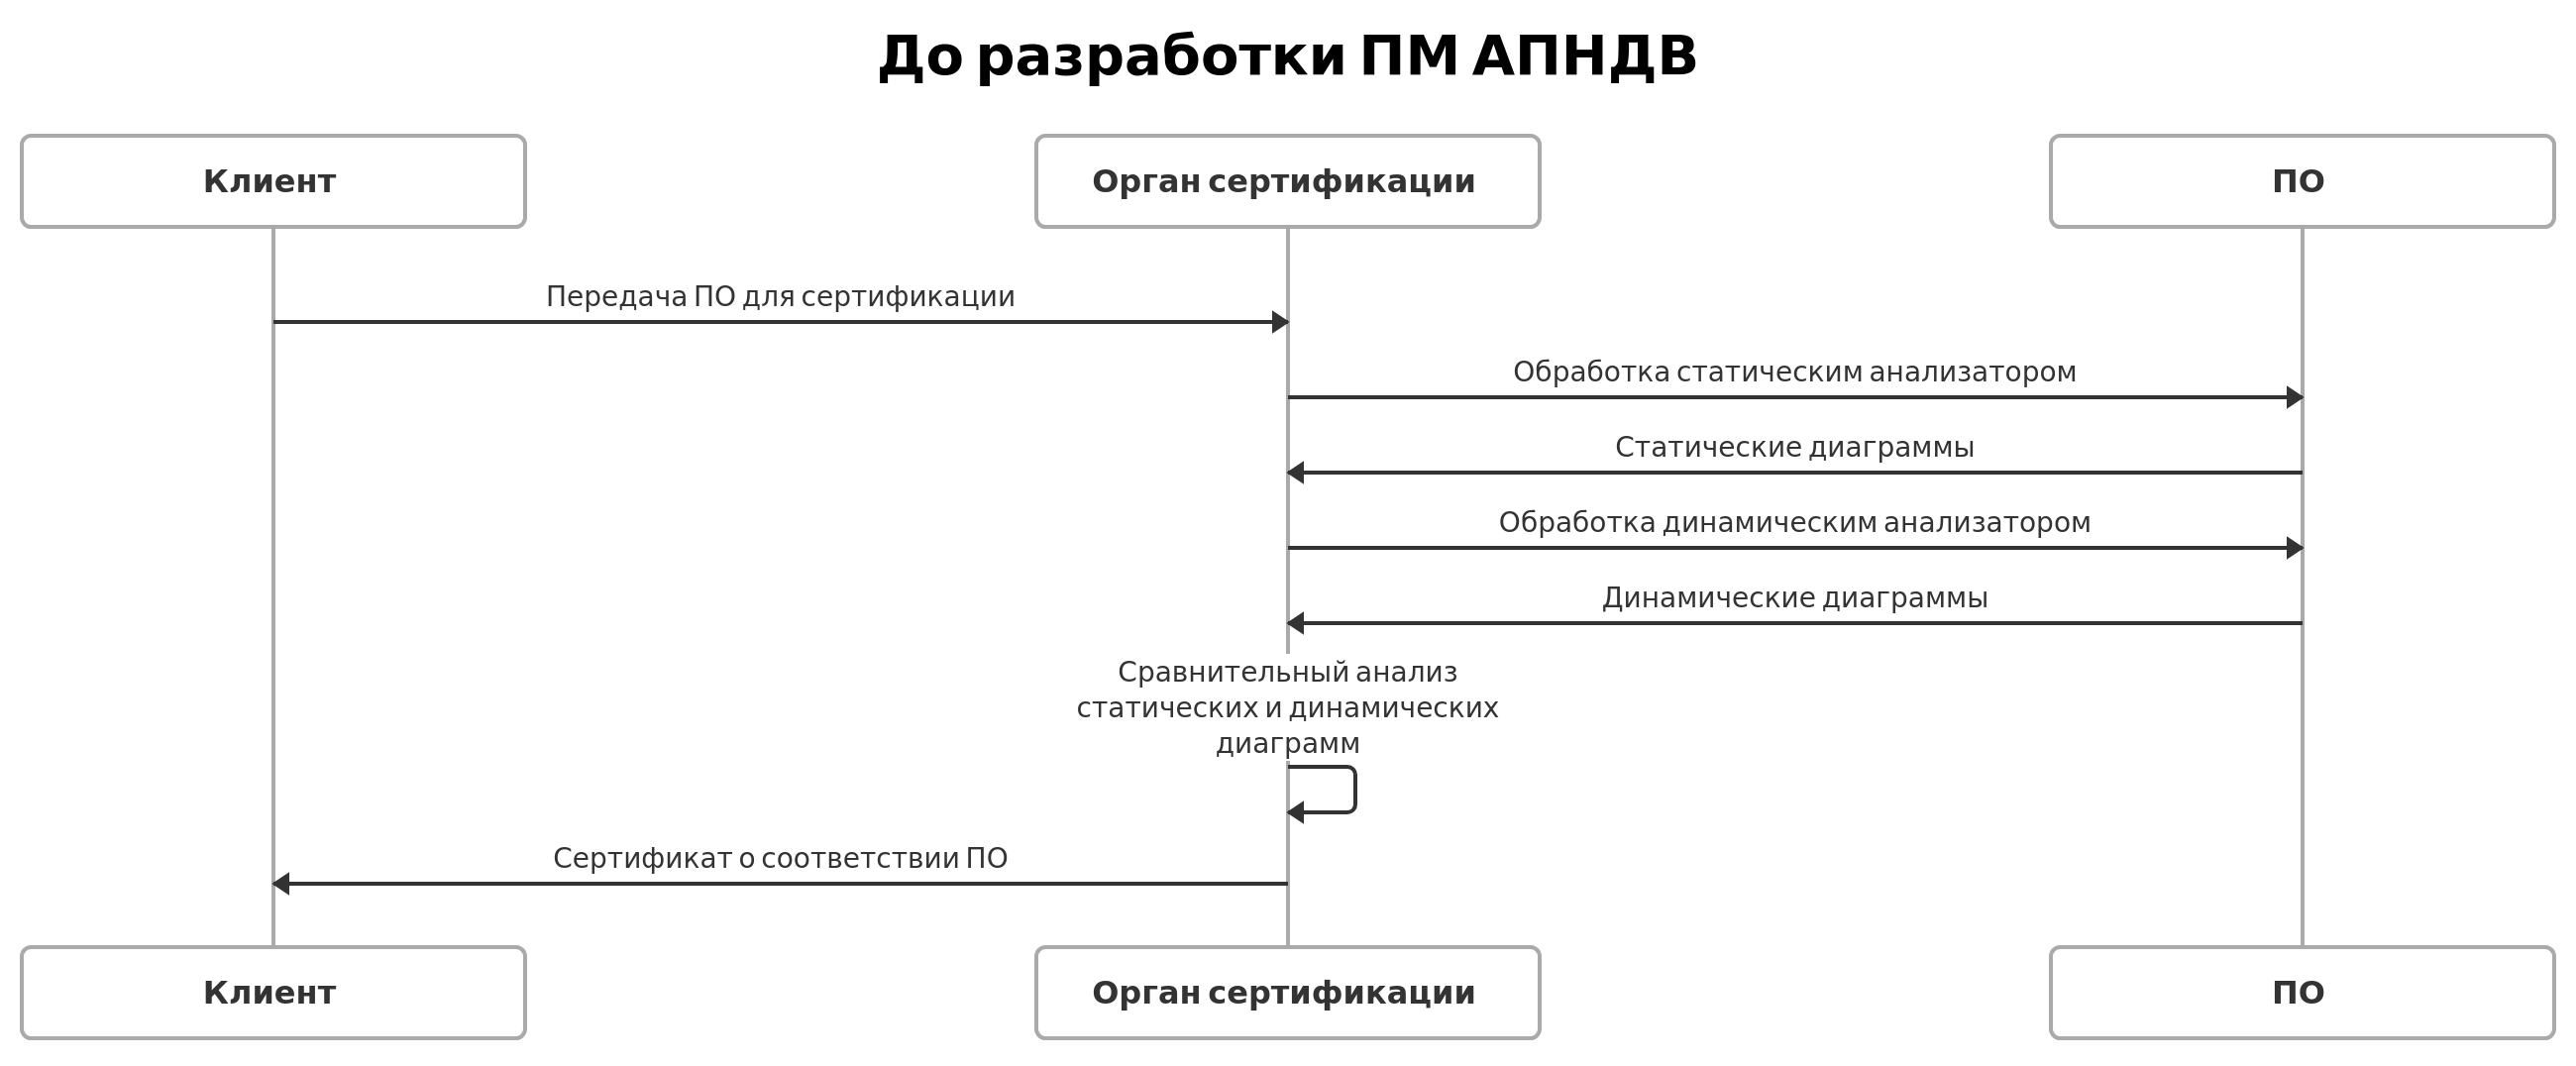
\includegraphics[width=\textwidth,height=\textheight,keepaspectratio]{images/uml_before_cropped.png}
    \caption{Процесс проведения сертификации раньше\label{fig:how-cert-was-before}}
\end{figure}

\begin{figure}[!htbp]
    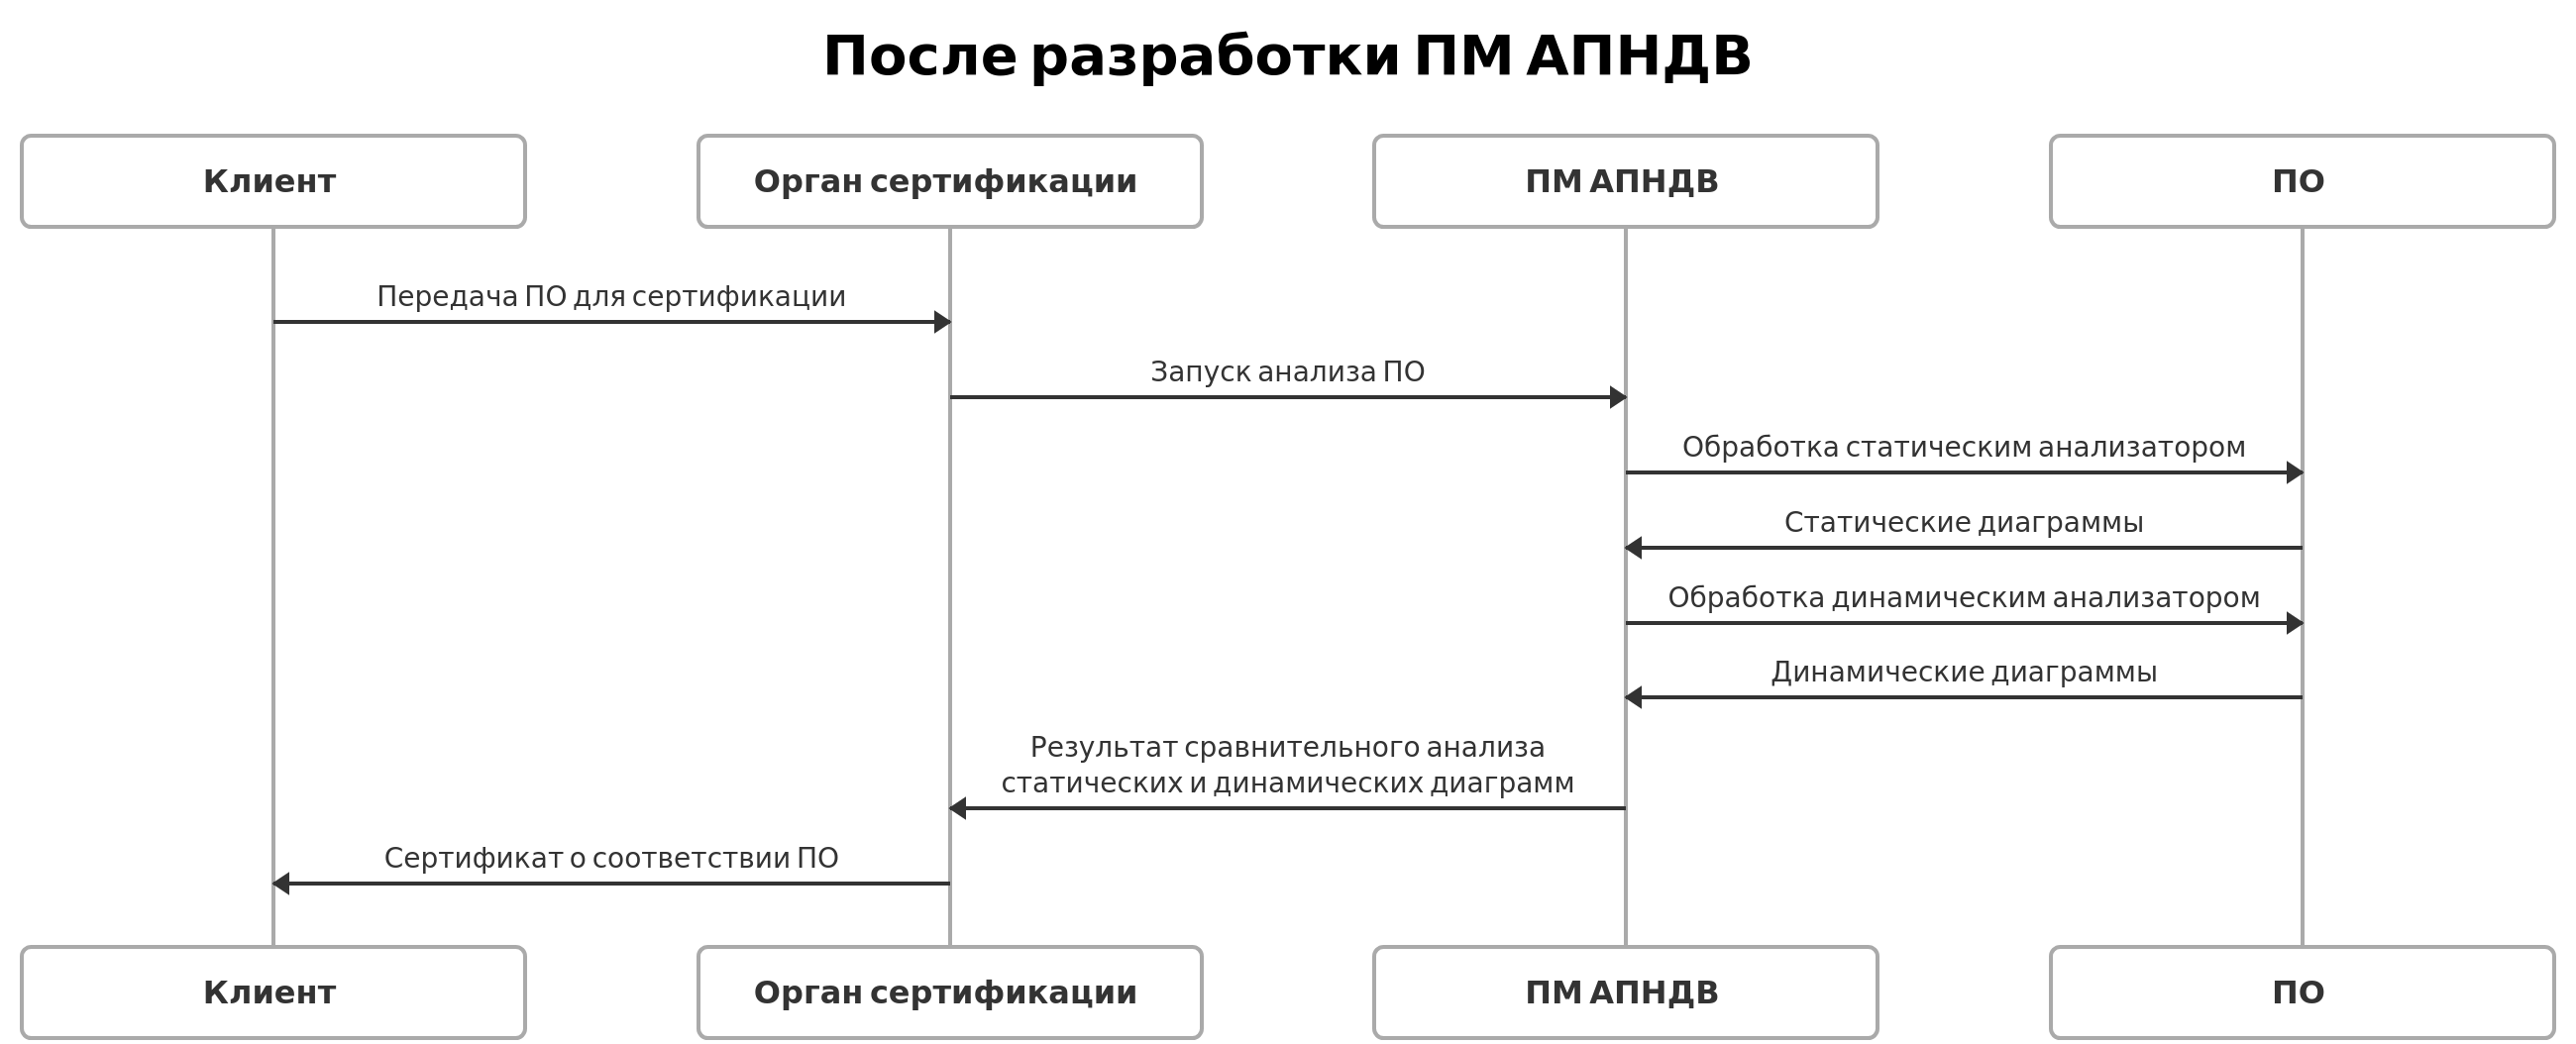
\includegraphics[width=\textwidth,height=\textheight,keepaspectratio]{images/uml_after_cropped.png}
    \caption{Процесс проведения сертификации с использованием {\ProgModule}\label{fig:how-cert-is-now}}
\end{figure}

\subsection{Сравнение статических анализаторов}\label{sec:ch1/sec3/sub1}
Статический анализ исходных кодов проводится без надобности сборки и запуска 
анализируемой программы. 

Статические анализаторы, в основном, явно или побочно используются разработчиками через программы-линтеры (\autoref{fig:vs-lint}) и компиляторы
для обнаружения нежелательного поведения или нарушения стиля программирования, не связанного с корректностью
исходного кода грамматике языка. 
Данные статические анализаторы будут сообщать, например, если выражение потенциально
может вызывать переполнение стека или условное выражение всегда будет исполнять только одну
из своих веток.

\begin{figure}[!htbp]
    \centerfloat{
        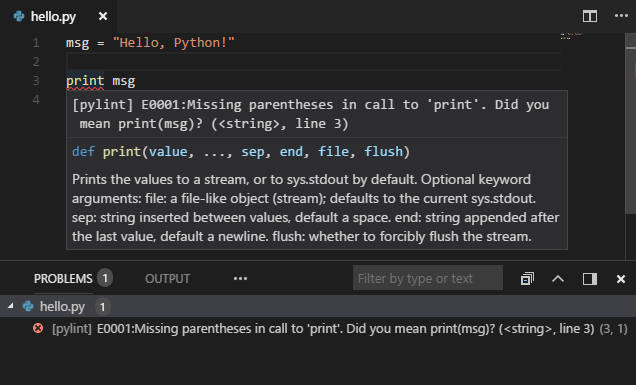
\includegraphics[width=\linewidth]{images/VSlint.png}
    }
    \caption{Линтер языка python в Visual Studio Code\label{fig:vs-lint}}
\end{figure}

Не смотря на всю полезность данных статических анализаторов, в контексте сертификации
программного обеспечения на НДВ они имеют малое практическое применение и
скорее относятся к повышению качества или читаемости кода.

Поэтому в таблице \ref{table:static-analyzers-comparsion} рассмотрим статические анализаторы, специализирующиеся на создании карт исходного кода.

{\small
    \setlength{\tabcolsep}{2pt}
    \begin{longtable}{*{5}{| c}|}
    \caption{\label{table:static-analyzers-comparsion}
           Сравнительная таблица статических анализаторов}\\
        \hline
        \diagbox[width=8cm]{Свойства}{Название программы}                 &
        \makecell{Microsoft\\Application\\Inspector}                      &
        \makecell{SCI\\Tools\\Understand \autocite{sci-tools-understand}} &
        \makecell{GNU cflow \autocite{gnu-cflow}}                         &
        \makecell{Kernel\\analyzer} \\
        \hline
        \makecell{Кроссплатформенность}             & \greencell{Да} & \greencell{Да} & \greencell{Да} & \greencell{Да}\\
        \hline
        \makecell{Открытость\\исходного кода}        & \greencell{Да} & \redcell{Нет}  & \greencell{Да} & \redcell{Нет} \\
        \hline
        \makecell{Препроцессирование\\кода C/C++}    & \redcell{Нет}  & \greencell{Да} & \greencell{Да} & \greencell{Да}\\
        \hline
        \makecell{Представление\\
                  препроцессорных директив как\\
                  вызов функций}                     & \redcell{Нет}  & \redcell{Нет}  & \greencell{Да} & \redcell{Нет} \\
        \hline
        \makecell{Создание графа вызовов}            & \redcell{Нет}  & \greencell{Да} & \greencell{Да} & \greencell{Да}\\
        \hline
        \makecell{Создание обратного\\графа вызовов} & \redcell{Нет}  & \greencell{Да} & \greencell{Да} & \redcell{Нет}  \\
        \hline
        \makecell{Бесплатность}                      & \greencell{Да} & \redcell{Нет}  & \greencell{Да} & \greencell{Да}\\
        \hline
        \makecell{Графический интерфейс}             & Нет            & Есть           & Нет            & Нет           \\
        \hline
    \end{longtable}
}

\subsubsection{Microsoft Application Inspector}\label{sec:ch1/sec3/sub1/sub1}

\begin{figure}[!htbp]
    \centerfloat{
        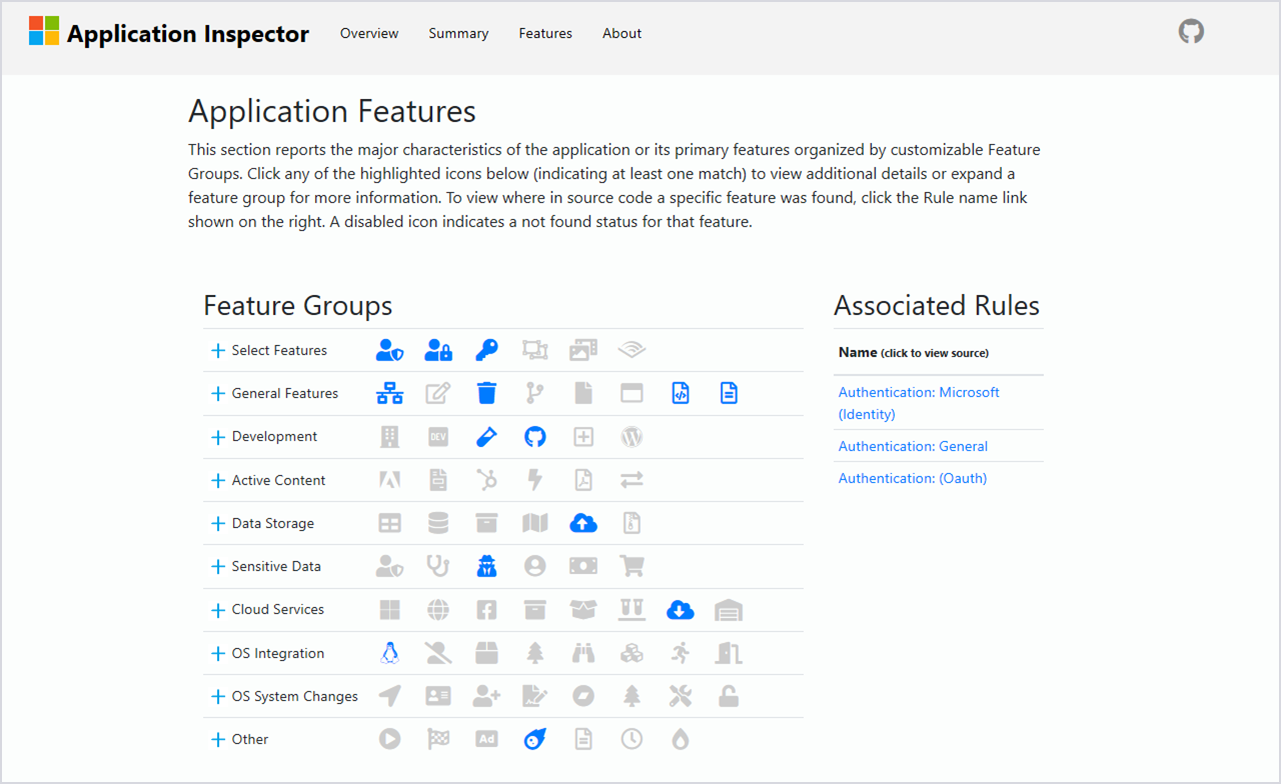
\includegraphics[width=\linewidth]{images/MSAppInspector.png}
    }
    \caption{Отчет Microsoft Application Inspector\label{fig:ms-app-inspector}}
\end{figure}
Задача Microsoft Application Inspector -- Систематическая и масштабируемая идентификация функций исходного кода.
Анализатор написан на .NET Core \autocite{net-core}, а это значит, что программа будет работать на всех платформах,
для которых реализован .NET Core: Windows, GNU/Linux и macOS.

Microsoft Application Inspector распознает паттерны поведения функций не только в 34 языках, 
но также и в их смешениях -- когда взаимодействующие части программы
написаны на разных языках.
Умеет замечать отличия в поведении между различными версиями инспектируемого 
программного модуля. 

Является бесплатным ПО, с открытым исходным кодом.
Позволяет защититься от НДВ только на переднем плане, так как анализирует исходные коды
подключенных модулей, но бессилен при появлении НДВ на этапе компиляции.

В качестве недостатков Microsoft Application Inspector можно 
отметить предметный анализ функций, который ничего не говорит 
о последовательности их вызова.

\subsubsection{SCI Tools Understand}\label{sec:ch1/sec3/sub1/sub2}
SCI Tools Understand -- кроссплатформенный, быстрый статический анализатор больших объемов кода,
имеющий хорошие возможности в визуализации отношений модулей программы,
имеет встроенный расчет различных метрик программного кода.

Поддерживает около 20 языков программирования, а также распознает код, написанный под разными 
стандартами.
Недостатки SCI Tools Understand -- платность и закрытый исходный код. Но купив лицензионную копию
программы, пользователь получает возможность писать скрипты манипуляции БД анализируемого проекта, 
генерирования отчетов и собственных метрик.

\subsubsection{GNU cflow}\label{sec:ch1/sec3/sub1/sub3}
Быстрый и минималистичный статический анализатор, с открытым исходным кодом,
позволяющий создавать как прямые, так и обратные графы вызовов. 
Командный интерфейс приближен к командному интерфейсу компилятора.
Поддерживает языки C и C++, а также LEX и YACC.
К достоинствам также можно отнести удобный и емкий формат отчета, который легко
разбирать регулярными выражениями.

\subsubsection{Kernel analyzer}\label{sec:ch1/sec3/sub1/sub3}
Статический анализ утилита анализа ядра проводит через
компиляцию исходного кода ядра компиляторами clang и gcc, с последующим
разбором сгенерированных ими абстрактных синтаксических деревьев,
что является гарантированно честным, но не самым производительным способом
генерации статических диаграмм.

Помимо статического и динамического Kernel analyzer анализа имеет сравнительный анализ,
а также команды для проверки специфических ситуаций,
таких как накапливание информации в ядре и 
трассирование процесса запуска системы.

\subsubsection{Вывод}\label{sec:ch1/sec3/sub1/sub4}
Из рассмотренных статических анализаторов, ни один не удовлетворяет всем требованиям,
что призван решить {\ProgModule}.
Так как {\ProgModule} ориентирован на анализ C/C++ программ, то проанализировав
\autoref{table:static-analyzers-comparsion} приходим к выводу, что для 
использования как составной части {\ProgModule}, функционал 
Microsoft Application Inspector не покрывает нужные сценарии использования, 
а SCI Tools Understand не подходит из-за своей закрытости и платности, Kernel analyzer -- узконаправленности.
Единственный возможнный выбор -- GNU cflow. 

\subsection{Сравнение динамических анализаторов}\label{sec:ch1/sec3/sub2}
Динамический анализ программного обеспечения может проводиться в реальном
или эмулированном окружении. Проведение динамического
анализа, требует тестирования максимального количества вариантов
ввода данных для прохождения исследуемой программой как можно большего количества путей генерации 
выходных данных.
Динамический анализ, необходимый в рамках сертификации программного обеспечения, может проводиться
программами различного назначения, до тех пор, пока программа, используемая как анализатор, умеет сама или побочно
создавать динамическую карту вызовов.

В таблице \ref{table:dynamic-analyzers-comparsion} рассмотрим программы, потенциально пригодные для проведения динамического
анализа.

{\small
    \setlength{\tabcolsep}{2pt}
    \begin{longtable}{*{5}{| c}|}
    \caption{\label{table:dynamic-analyzers-comparsion}
           Сравнительная таблица программ для динамического анализа}\\
        \hline
        \diagbox[width=8cm]{Свойства}{Название программы} &
        \makecell{Gcov \autocite{gcov}}                   &
        \makecell{GDB \autocite{gdb}}                     &
        \makecell{QEMU \autocite{qemu}}                   &
        \makecell{Kernel\\analyzer}                   \\
        \hline
        \makecell{Кроссплатформенность}             & \greencell{Да} & \greencell{Да} & \greencell{Да} & \greencell{Да} \\
        \hline
        \makecell{Открытость\\исходного кода}        & \greencell{Да} & \greencell{Да} & \greencell{Да} & \redcell{Нет} \\
        \hline
        \makecell{Возможность\\анализировать память} & \redcell{Нет} & \greencell{Да} & \greencell{Да} & \greencell{Да} \\
        \hline
        \makecell{Возможность\\программно управлять} & \redcell{Нет} & \greencell{Да} & \greencell{Да} & \redcell{Нет} \\
        \hline
        \makecell{Возможность\\создавать\\
                  собственные команды}               & \redcell{Нет} & \greencell{Да} & \redcell{Нет} & \redcell{Нет} \\
        \hline
        \makecell{Возможность удаленной\\
                  отладки}                           & \redcell{Нет} & \greencell{Да} & \redcell{Нет} & \redcell{Нет} \\
        \hline
        \makecell{Бесплатность}                      & \greencell{Да} & \greencell{Да} & \greencell{Да} & \greencell{Да} \\
        \hline
        \makecell{Поддержка отладки\\
                  программ, написанных\\
                  не для x86 архитектуры}            & \greencell{Да} & \greencell{Да} & \greencell{Да} & \greencell{Да} \\
        \hline
        \makecell{Графический интерфейс}             & Есть & Есть & Есть & Нет \\
        \hline
    \end{longtable}
}

\subsubsection{Gcov}\label{sec:ch1/sec3/sub2/sub1}
Утилита для создания покрытия кода, входит в пакет GCC (GNU Compiler Collection).
Генерирует новые исходные файлы, в которых на каждой строчке указано количество
раз, сколько была вызвана та или иная функция. Больше не генерирует никакой информации,
и работает только с программами, скомпилированными с помощью GCC. 
С помощью графического интерфейса lcov можно создавать html-отчеты (\autoref{fig:lcov}) о
пройденных трассах.

\begin{figure}[!htbp]
    \centerfloat{
        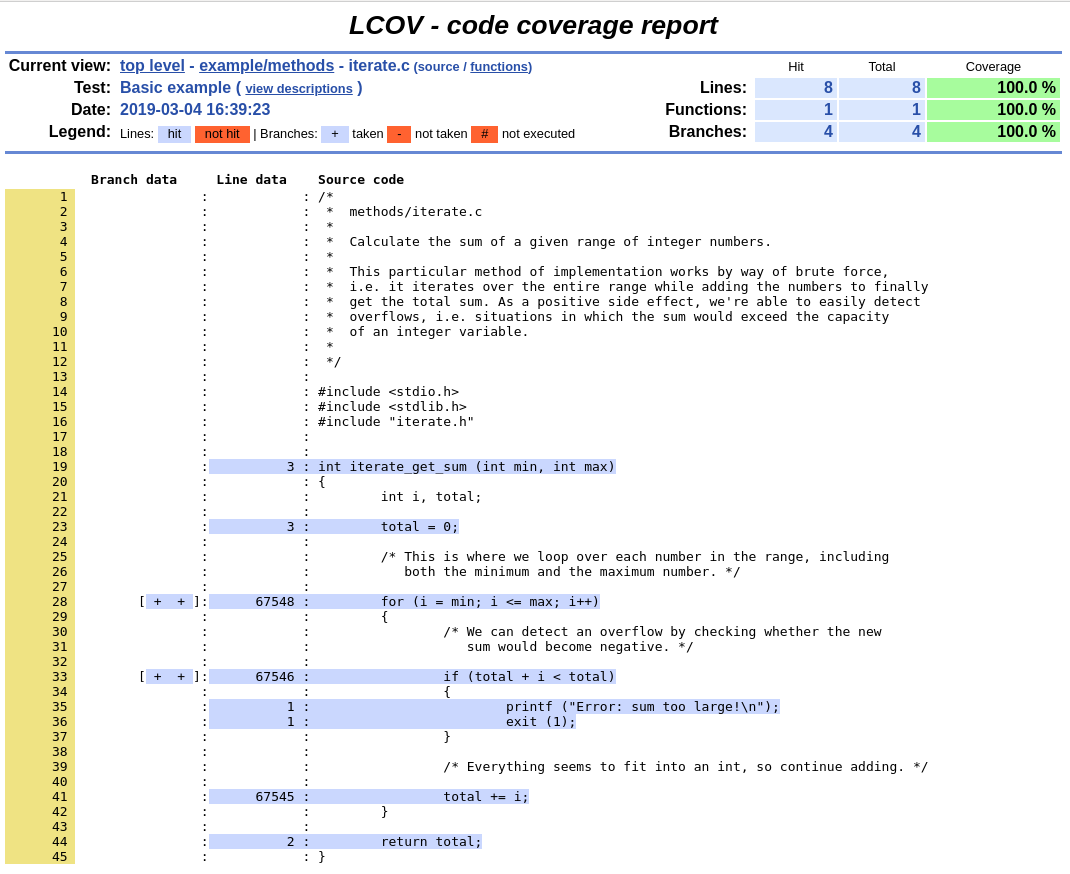
\includegraphics[width=\linewidth]{images/lcov.png}
    }
    \caption{Отчет lcov\label{fig:lcov}}
\end{figure}

\subsubsection{GNU Debugger}\label{sec:ch1/sec3/sub2/sub2}
Отладчик GDB (\autoref{fig:gdb-tui}) впервые увидел свет в 1986 году и за прошедшие годы обзавелся
большим количеством поддерживаемых архитектур процессоров, самые известные, из них:
\begin{itemize}
    \item Alpha;
    \item ARM;
    \item AVR;
    \item H8/300;
    \item Altera Nios/Nios II;
    \item System/370;
    \item System 390;
    \item X86 и X86-64;
    \item IA-64 "Itanium";
    \item Motorola 68000;
    \item MIPS;
    \item PA-RISC;
    \item PowerPC;
    \item SuperH;
    \item SPARC;
    \item VAX.
\end{itemize}
Существует под все популярные операционные системы. Часто используется в различных IDE в качестве
отладчика из за своей надежности и текстового интерфейса GDB/MI (MI расшифровывается как Machine
Interface), позволяющего использовать отладчик в качестве компонента некой большой системы.
К достоинствам можно отнести возможность описания сценария отладки в командном файле,
с последующим исполнением его GDB, расширение возможностей отладчика через программирование
на встроенном интерпретаторе python, создание макрокоманд с помощью уже существующих,
а также удаленную отладку.
\begin{figure}[!htbp]
    \centerfloat{
        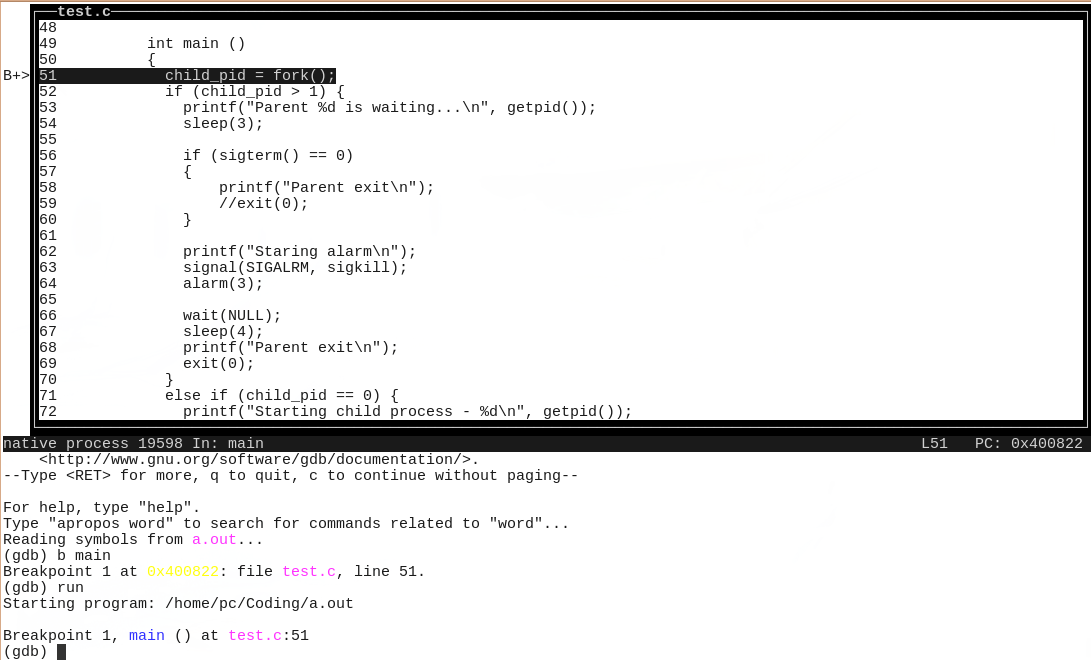
\includegraphics[width=\linewidth]{images/GDB.png}
    }
    \caption{Терминальный интерфейс GDB \label{fig:gdb-tui}}
\end{figure}

\subsubsection{QEMU}\label{sec:ch1/sec3/sub2/sub3}
\begin{figure}[!htbp]
    \centerfloat{
        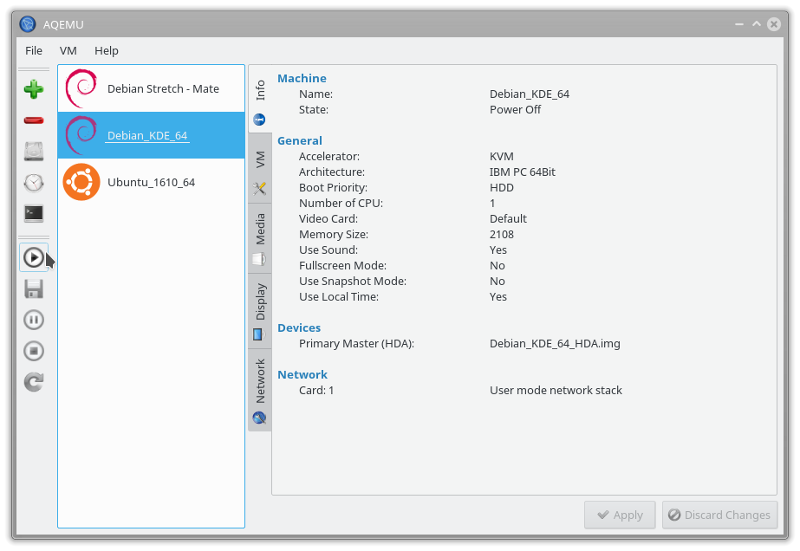
\includegraphics[width=\linewidth]{images/QEMU_GUI.png}
    }
    \caption{Графическая оболочка AQEMU для эмулятора QEMU\label{fig:aqemu}}
\end{figure}
QEMU -- Быстрый эмулятор процессоров, поддерживает множество просессорных архитектур,
предоставляет возможность сохранять сгенерированный машинный код. Существует
под все популярные операционные системы.
Помимо эмуляции процессора, QEMU (\autoref{fig:aqemu}) может эмулировать и периферийные устройства:
сетевые карты, жесткие диски, видео карты, PCI, USB и др.
К недостаткам можно отнести медленную, по сравнению с отладчиком работу,
так как эмулятору приходится преобразовывать каждую инструкцию запущенной программы
в машинный код процессора, на котором он запущен.

Работает это следующим образом:
инструкции запущенной внутри QEMU программы конвертируются в промежуточный,
платформонезависимый код при помощи интерпретатора TCG (Tiny Code Generator),
затем этот платформонезависимый код компилируется уже в целевые машинные инструкции.

\subsubsection{Kernel analyzer}\label{sec:ch1/sec3/sub1/sub3}
В динамическом анализе утилита полагается на QEMU и проводит его через
разбор call-инструкций в скомпилированном TCG коде.

\subsubsection{Вывод}\label{sec:ch1/sec3/sub2/sub4}
Так как для более точного выполнения задачи сертификации будет полезно получать
информацию времени выполнения программы, такую, как:
\begin{enumerate}[label={\arabic*)}]
    \item значения регистров перед вызовом функции;
    \item состояние стека перед вызовом функции;
    \item стек вызовов;
    \item экспертиза результатов;
    \item информацию о сегментах и функциях, определенных в них.
\end{enumerate}
А также расширять возможность динамического анализатора с помощью скриптов,
то из \autoref{table:dynamic-analyzers-comparsion} следует, что
удобнее всего это можно будет сделать с помощью отладчика GDB,
нежели эмулятора QEMU или генератора покрытия кода Gcov. Kernel analyzer --
по тем же причинам, что и QEMU.


\section{Постановка задачи ВКР}\label{sec:ch1/sec4}
На основе изложенного в \autoref{sec:ch1/sec1}-\autoref{sec:ch1/sec3} сформированы
следующая цель и задачи ВКР.
Цель: ускорение процедуры сертификации программного обеспечения, написанного
на языках C и C++.

Задачи:
\begin{enumerate}[label={\arabic*)}]
    \item исследование предметной области;
    \item сравнительный анализ существующих программных решений;
    \item выбор языка и среды разработки;
    \item разработка схемы данных {\ProgModule};
    \item разработка схемы алгоритма {\ProgModule};
    \item программная реализация {\ProgModule};
    \item отладка и тестирование {\ProgModule};
    \item разработка руководства оператора {\ProgModule}.
\end{enumerate}

\section*{Выводы по разделу}\label{sec:ch1/sec5}
\addcontentsline{toc}{section}{Выводы по разделу}
В исследовательском разделе была рассмотрена предметная область процесса
сертификации программного обеспечения, теоретические и нормативные-правовые 
обоснования необходимости проведения данной процедуры, а также представлены
последствия игнорирования возможности внедрения НДВ  через доверенные программы --
компиляторы.

Проведен анализ существующих решений данной проблемы, из которого был сделан
вывод о том, что программы, аналогичной по универсальности {\ProgModule} нет на рынке.

Выбраны сторонние свободные программы в качестве компонентов {\ProgModule}.

Обоснована актуальность разработки {\ProgModule}.

Поставлены задачи для дальнейшей разработки {\ProgModule}.
